

\section*{Part \uppercase\expandafter{\romannumeral2} Proposal of the Individual Project}
\addcontentsline{toc}{section}{Part \uppercase\expandafter{\romannumeral2} Proposal of the Individual Project} 
\setcounter{section}{2}
\setcounter{subsection}{0}

%  -----  2.1
\subsection{Significance and Relevance of the Individual Project to the Group Project}

\subsubsection{Complementary Role}
My individual project significantly addresses the perception, input game values, plan creation, and interactive components of the AI agent system. 
Concentrating on the agent's perception within the external gaming environment and harnessing this information to drive decision-making, 
my contribution largely enhances the narrative of the metaverse game. 
Here, AI agents actively interact with users, cultivating an immersive and engaging storytelling adventure.

Recent advancements in natural language and Large Language Models (LLMs) have enabled AI agents to simulate human-like interactions within virtual worlds. 
However, these interactions still face limitations in complexity and flexibility, particularly in scenarios involving multiple characters and novel objects\cite{liang2023tachikuma}. 
In addition, although large language models (LLM) have demonstrated extraordinary potential for natural language dialogues and assisted resolution of real-world tasks, 
it is difficult to accomplish complex simulation and interaction tasks with only large language models for natural language interaction in game or application level scenarios involving multi-intelligence interactions in narrative environments.

To address these challenges, my project implements the dynamic narrative component at the core of the group's project by designing and developing the foundational ai agent system framework in a way that fully incorporates the natural language understanding and generation capabilities of large language models and multimodal technology.
One of the most important gaps to fill is the functional gap between natural language understanding and generation from large language models to games, especially metaverse narrative games, because large language models naturally have the ability to understand and generate natural language, and can realize fluent and even customized stylized dialogues, 
but they cannot complete the necessary functions of perception, planning, decision-making, and interaction of the game characters,which cannot rely on the language models alone. 
There is a research to suggest that large language models, though not sufficient by themselves, open up a new angle for creating believable agents when leveraged using the appropriate architecture\cite{park2023generative}. 

Storytelling in games has historically been the purview of the human designer. Interactive Narrative as a form of interactive digital entertainment in which some—or all—of the responsibility for managing the player’s narrative experience in the hands of an intelligent, autonomous system\cite{riedl2012interactive}. 
Currently, there is little understanding of how to instill narrative intelligence, i.e., the ability to represent and reason about storytelling, into game systems driven by large language models. 
As a result, there are many open-ended research questions on how to enable computational systems to reason about narratives and manage the player's interactive experience in virtual worlds. 
What is certain, however, is that there is a considerable functional gap between the large language model, or the multimodal large language model (MLLM), and direct narrative design, a good large language model narrative system can act as a bridge between the user, the large language model, and the narrative content, 
expanding the possibilities of natural language generation into a source of immersion in the narrative experience, thus avoid the tedious user-centered interactive text dialogue experience, 
and let users immerse into the narrative role to experience the carefully designed creative narrative content.

In conclusion, my individual project not only provides a foundational and innovative AI agent system framework but also brings a unique perspective from the realm of Human-Computer Interaction and Human-AI Interaction. 
By addressing the nuances of user experience and collaborative interactions, my work enriches the collective effort, contributing to the realization of the group project's vision of a technologically advanced, user-centric, and creatively immersive metaverse campus community.

\subsubsection{Value Addition}
My individual project holds significant value within the group project, particularly in the development of critical components that shape the AI agent system framework for metaverse narrative game. 
My project intricately addresses agent perception, game values, planning, decision-making, and interactions, reflecting a holistic approach to crafting a sophisticated and user-centric AI-driven storytelling experience. 
The distinctive expertise my project brings to the team project lies in the domains of Human-Computer Interaction and Human-AI Interaction. 
This expertise ensures that the perceptual interaction system is not only technologically advanced but also aligned with user needs and preferences. 
By infusing HCI methods into the project, my project contributes to a more intuitive and engaging metaverse narrative game, fostering a user-centered design approach.

Moreover, my project delves into the complexities of multi-player interactions and the integration of multiple AI agents, 
introducing a collaborative narrative dynamic. This aspect enhances user engagement, creating an immersive environment where users actively participate in shaping the overarching storyline. 
One of the key strengths of my project lies in its ability to optimize the potentials of Large Language Models (LLM) and Multimodal Large Language Models (MLLM) in interactive narrative content. 
Decision-making processes and reflective mechanisms ensure a seamless integration of these advanced AI models, resulting in a metaverse narrative game that leverages the strengths of cutting-edge technology for an innovative and captivating storytelling experience.

Additionally, my background in software engineering and game development further enriches the group project. 
This practical knowledge contributes to the overall development and presentation of the metaverse narrative game, ensuring a robust implementation that adheres to industry standards and practices. 
My proficiency in software development complements the team's efforts, enhancing the efficiency and progress of the broader research and development process.

My individual project serves as a cornerstone in creating a technologically advanced, user-centric, and collaborative metaverse narrative game. 
The value added lies not only in the development of critical components but also in the infusion of HCI expertise, multi-player interactions, optimal utilization of advanced AI models, and practical software development knowledge. 
My multifaceted contributions contribute significantly to the realization of the group project's vision of a groundbreaking AI agent-driven storytelling experience within the metaverse campus community.

\subsubsection{Interdependence}
My individual project, centered on the development of the multi-AI agent and multi-player perceptual interaction system, serves as a cornerstone in the collaborative effort of our group project. 
The interconnected nature of my project with others within the team project showcases a harmonious synergy that enhances the overall metaverse narrative game system.

Zhihan GUO's project, which delves into memory generation and decision-making of AI agents in story-telling game, 
forms a crucial connection with my work. The memory module in our AI agent system architecture relies heavily on GUO's multimodal large language model memory unit, significantly influencing the immersion of our AI agent system, especially the decision-making capability of the AI agent. 
The integration of memory generation from GUO's module becomes pivotal in shaping the dynamic and adaptive decision-making processes within the metaverse. 
Additionally, my project influences GUO's work by providing the necessary information processed through perceptual interactions, creating a reciprocal relationship that strengthens both components.

Furthermore, the collaborative connection extends to Yuelu LI's project, which explores interactive storytelling with AI agent intervention. 
LI's narrative elements, including scenes, characters, and plots, are intricately woven into my design. 
The decision-making function and interactions crafted not only considers GUO's memory module but also serves the narrative elements envisioned by LI. 
This interdependence ensures that the AI agent's decisions and actions align seamlessly with the dynamic narrative envisioned by LI, offering users a rich and engaging storytelling experience.

Moreover, Peixian MA's optimized model interface, providing information processing functions, plays a central role in influencing my project. 
MA's interface becomes the processing core, shaping the functionalities of my interaction and any other modules. 
My project, in turn, contributes to the optimization of the model interface by providing valuable insights and requirements for effective perceptual interactions and decision-making in the metaverse.

%  -----  2.2
\subsection{Statement of the Individual Project in Details}

\subsubsection{Literature/Market Review and Problem Definition}

\textbf{Market Review}\quad
Emerging as an intriguing concept, the metaverse points to a virtual universe where users can actively engage with others and their surroundings in real-time. 
Metaverse industry has seen significant growth recently, driven by the surge in virtual reality technologies. 
Such advancements have enabled the development of incredibly immersive and engaging digital landscapes. 
The Metaverse Market is not just introducing novel means of conducting business or socializing, but also holds the potential to transform our perspective of the Internet and digital technology. 
Additionally, metaverses offer innovative means for people to connect, fostering communities in unprecedented ways. The ripple effects could substantially influence a variety of sectors from education to politics. 
In essence, the metaverse represents an exhilarating new horizon, teeming with limitless opportunities for innovation, creativity, and exploration.
According to Bloomberg, the Metaverse Market, which was a \$500 billion in 2020 (when virtual worlds started to gain popularity) will be a \$800 billion dollar market by 2024. This represents an annual compound growth rate of 13.1\% based on Bloomberg’s analysis\cite{Tech_undated-bj}. 
As per the SNS Insider Research, the Metaverse Market size was valued at US\$ 57.12 Bn in 2022, and is Projected to reach US\$ 796 Bn by 2030, with growing healthy CAGR of 39\% over the Forecast Period 2023-2030\cite{Metaverse_Market}. 
\begin{figure}
    \centering
    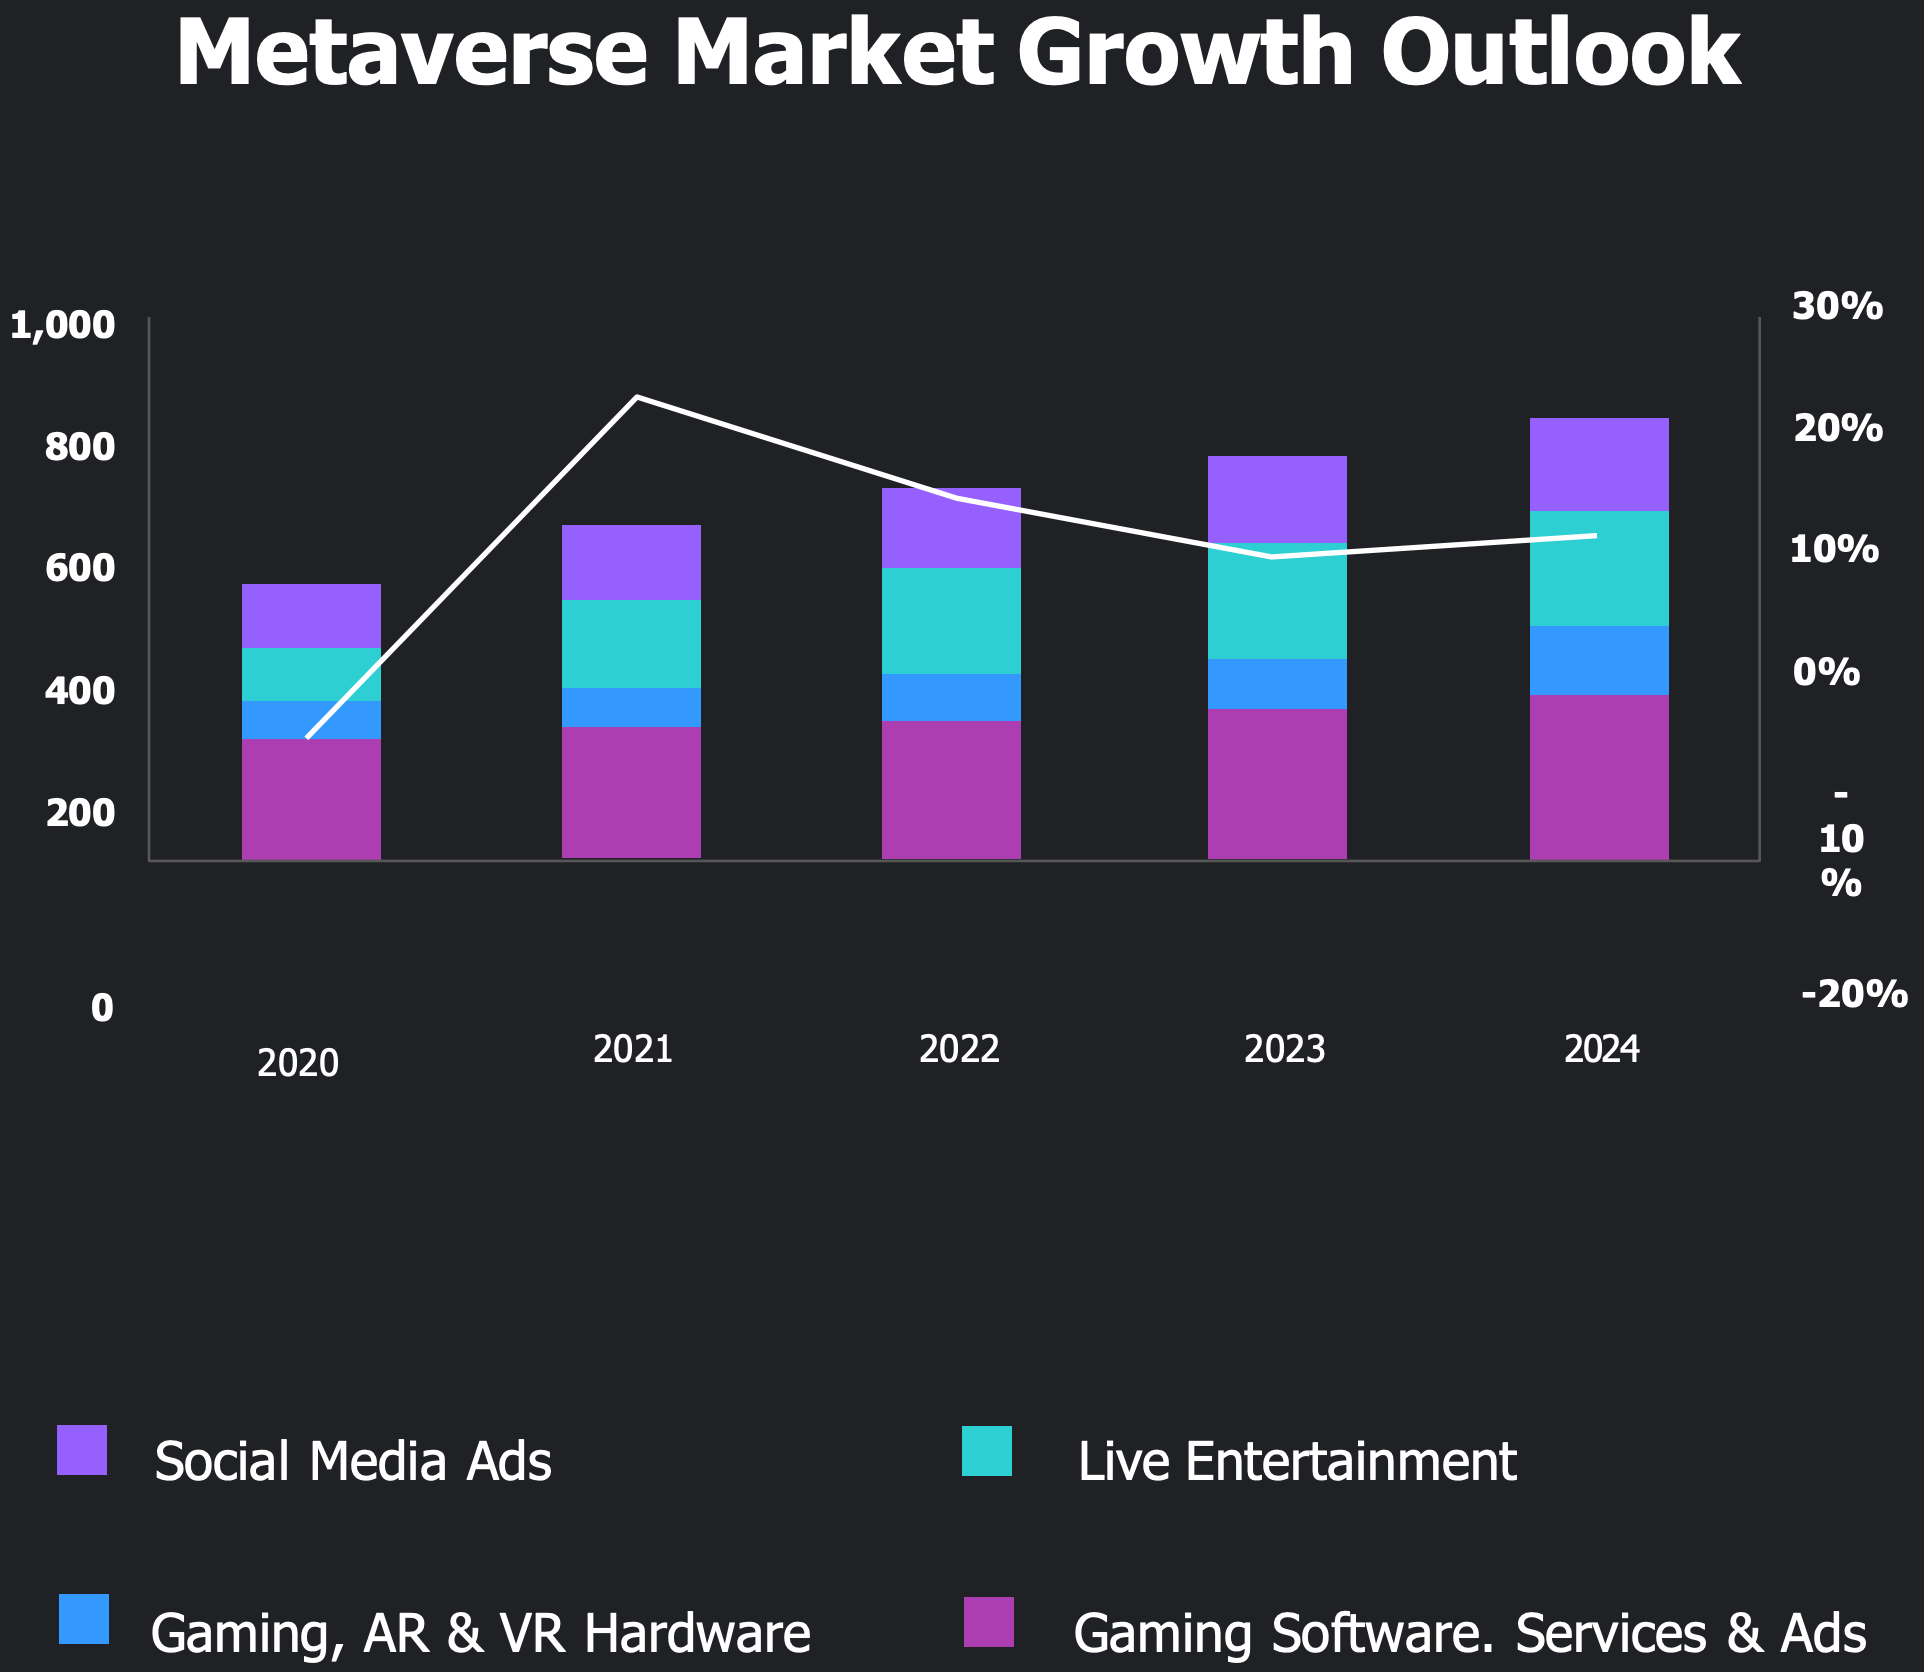
\includegraphics[width=0.8\textwidth]{image/MetaverseMarketOutlook.png}
    \caption{Metaverse Market Growth Outlook}
  \label{fig:Market}
\end{figure}
Artificial intelligence in games involves responsive and adaptive video game environments. 
NPCs or non-player characters are often the source of these AI-driven interactive experiences. 
They behave intelligently or imaginatively, just like human gamers. Artificial intelligence is the mechanism that determines how NPCs act in the virtual environment. 
In addition to NPCs, AI in games provides better user experience and other features such as high-quality graphics and animations.
The Artificial Intelligence (AI) in Games Market size is anticipated to experience substantial growth, projected at a Compound Annual Growth Rate CAGR of 24.65\% from 2023 to 2028, with an estimated market size to increase by USD 4.50 billion. 
This market is structured in a fragmented manner, exhibiting a Year-over-Year (YoY) growth of 22.96\% in 2023-2024. 
In the regional breakdown, this analysis includes North America, APAC, Europe, South America, and Middle East and Africa, with North America contributing significantly, standing at 44\%. 
Key countries propelling this market include the US, China, South Korea, Taiwan, and Japan\cite{AIGAME_Market_research}. 

But traditional NPCs are often programmed and limited to simple, repetitive patterns of conversation and behavior that can be boring.
That's why Inworld surveyed 1,002 U.S. gamers to better understand what different types of players love, hate, and secretly desire from NPCs. 
The report\cite{Inworld_Research} shows that the vast majority of players recognize the important role of NPCs, with 84\% saying they make a substantial difference to their gaming experience. 
52\% said they dislike repetitive NPC conversations, and the repetitive motions and maladaptive abilities of NPCs are among their least favorite aspects. Respondents like the idea of advanced AI NPCs - 79\% of respondents said they are excited about AI NPCs, 88\% believe AI NPCs will make games more immersive, and 78\% said they would spend more time playing games that include advanced AI characters. 
78\% of gamers would spend more time playing games, and 79\% would be more willing to buy games with intelligent NPCs. What's more, 81\% of gamers are willing to pay more for games with advanced AI NPCs. 

\textbf{Large Language Models in Game}\quad
The literature review begins with an exploration of the utilization of Large Language Models (LLMs) in the realm of gaming.
Thus far, generative AI models such as GPT-4 have exhibited the capacity to revolutionize numerous facets of our existence, particularly through their ability to emulate human language. This offers many individuals optimism for more refined simulations of human behavior or non-playable characters (NPCs).
The advent of LLMs has significantly transformed the gaming landscape, introducing a new dimension of interaction and engagement. These models, equipped with the ability to understand and generate natural language and human-like text, have been employed to create dynamic narratives, enhance player immersion, and facilitate complex in-game conversations.
For example, Tachikuma from Liang et al.\cite{liang_tachikuma_2023} drawing inspiration from Tabletop Role-Playing Games (TRPGs), comprising a Multiple character and novel Object based interaction Estimation (MOE) task for evaluating LLMs’ understanding over multiple-role and objects interactions via skill check answering.
Wu et al. explore the application of LLMs in "Jubensha" (Chinese murder mystery role-playing games), a novel area in AI-driven gaming, while also serves game features specifically designed to improve the performance of AI agents in key areas such as information gathering, murderer detection and logical reasoning\cite{wu_deciphering_2023}. 
Relatively earlier studies have focused more on experiments with popular analog language games between multiple intelligent agents, such as \textit{Werewolf} or \textit{Mafia-like} Game\cite{xu_language_2023, xu_exploring_2023, kim_generative_2023}.
Xu et al.\cite{xu_language_2023} propose a new framework powered by reinforcement learning (RL) to develop strategic language agents, i.e., LLM-based agents with strategic thinking ability, for a popular language game, \textit{Werewolf}, 
while Xu et al.\cite{xu_exploring_2023} demonstrates that LLMs can effectively play \textit{Werewolf} game and emerge strategic behaviors without tuning the parameters. 
Kim et al.\cite{kim_generative_2023} mainly focus on the gap between different generative models in \textit{Mafia-like} game. 
Suspicion-Agent by Guo et al.\cite{guo_suspicion-agent_2023} leverages GPT-4’s capabilities to perform in imperfect information games and find GPT-4 exhibits a robust high-order theory of mind (ToM) capacity, meaning it can understand others and deliberately influence their behavior. 
Other research involves abstract games such as the Prisoner's Dilemma, a game-theoretic simulation scenario\cite{akata_playing_2023, mao_alympics_2023, lore_strategic_2023}. 
There has also been research utilizing LLMs to generate game content and levels, Todd et al.\cite{todd_level_2023} use of LLMs to generate levels for the game \textit{Sokoban}. 
LingoLand using generative machine learning and immersing people in foreign language learning environments designed to mimic real scenarios\cite{seow_lingoland_2023}.

\textbf{Decision-making and planning with Large Language Models}\quad
LLMs intersect with decision-making and planning mechanisms as well. 
LLMs are more than just conversational agents - they are also used to model intelligent behavior and make decisions based on the contextual environment. 
More sophisticated AI personas developed by merging LLMs with decision-making processes are able to dynamically react and adapt to user behavior. 
LLMs have showcased remarkable performance in natural language processing tasks, and have been tested to perform another widely-studied crucial aspect of AI agents, namely, sequential decision-making or planning.
Preliminary studies have shown that in certain everyday areas, LLMs are able to propose sound action plans\cite{ahn2022can, huang2022language}, and 
InstructGPT\cite{ouyang2022training} and Codex\cite{chen2021evaluating} can be used as zeroshot planners to generate sub-goal sequences for various tasks in embodied environments.
However, the correctness and enforceability of these plans are often limited. 
Guan et al.\cite{guan_leveraging_2023} constructs an explicit world (domain) model in planning domain definition language (PDDL) and then uses it to plan with sound domain-independent planners while employ LLMs as an interface between PDDL and sources of corrective feedback.
Wang et al.\cite{wang_describe_2023} proposed “Describe, Explain, Plan and Select” (DEPS), which integrating description of the plan execution process and providing self-explanation of feedback when encountering failures during the extended planning phases and designed a trainable goal selector.
ChoiceMates\cite{park_choicemates_2023} is a system that enables conversations with a dynamic set of LLM-powered agents for a holistic domain understanding and efficient discovery and management of information to make decisions.
Lin et al.\cite{lin2023decision} designed agents that can collaborate with one or multiple humans, determining the shared knowledge among the cooperative partners, identifying which information is relevant to decisionmaking, posing questions, and engaging in reasoning to complete tasks such as allocation, planning, and scheduling.
During the process of plan formulation, agents generally decompose an overarching task into numerous sub-tasks, and various approaches have been proposed in this phase. Notably, some works advocate for LLM-based agents to decompose problems comprehensively in one go, formulating a complete plan at once and then executing it sequentially\cite{zhou2022least}. 
In contrast, other studies like the CoT-series employ an adaptive strategy, where they plan and address sub-tasks one at a time, allowing for more fluidity in handling intricate tasks in their entirety\cite{wei2022chain}.

\textbf{Multi-agent system simulating human behaviors}\quad
\begin{figure}
    \centering
    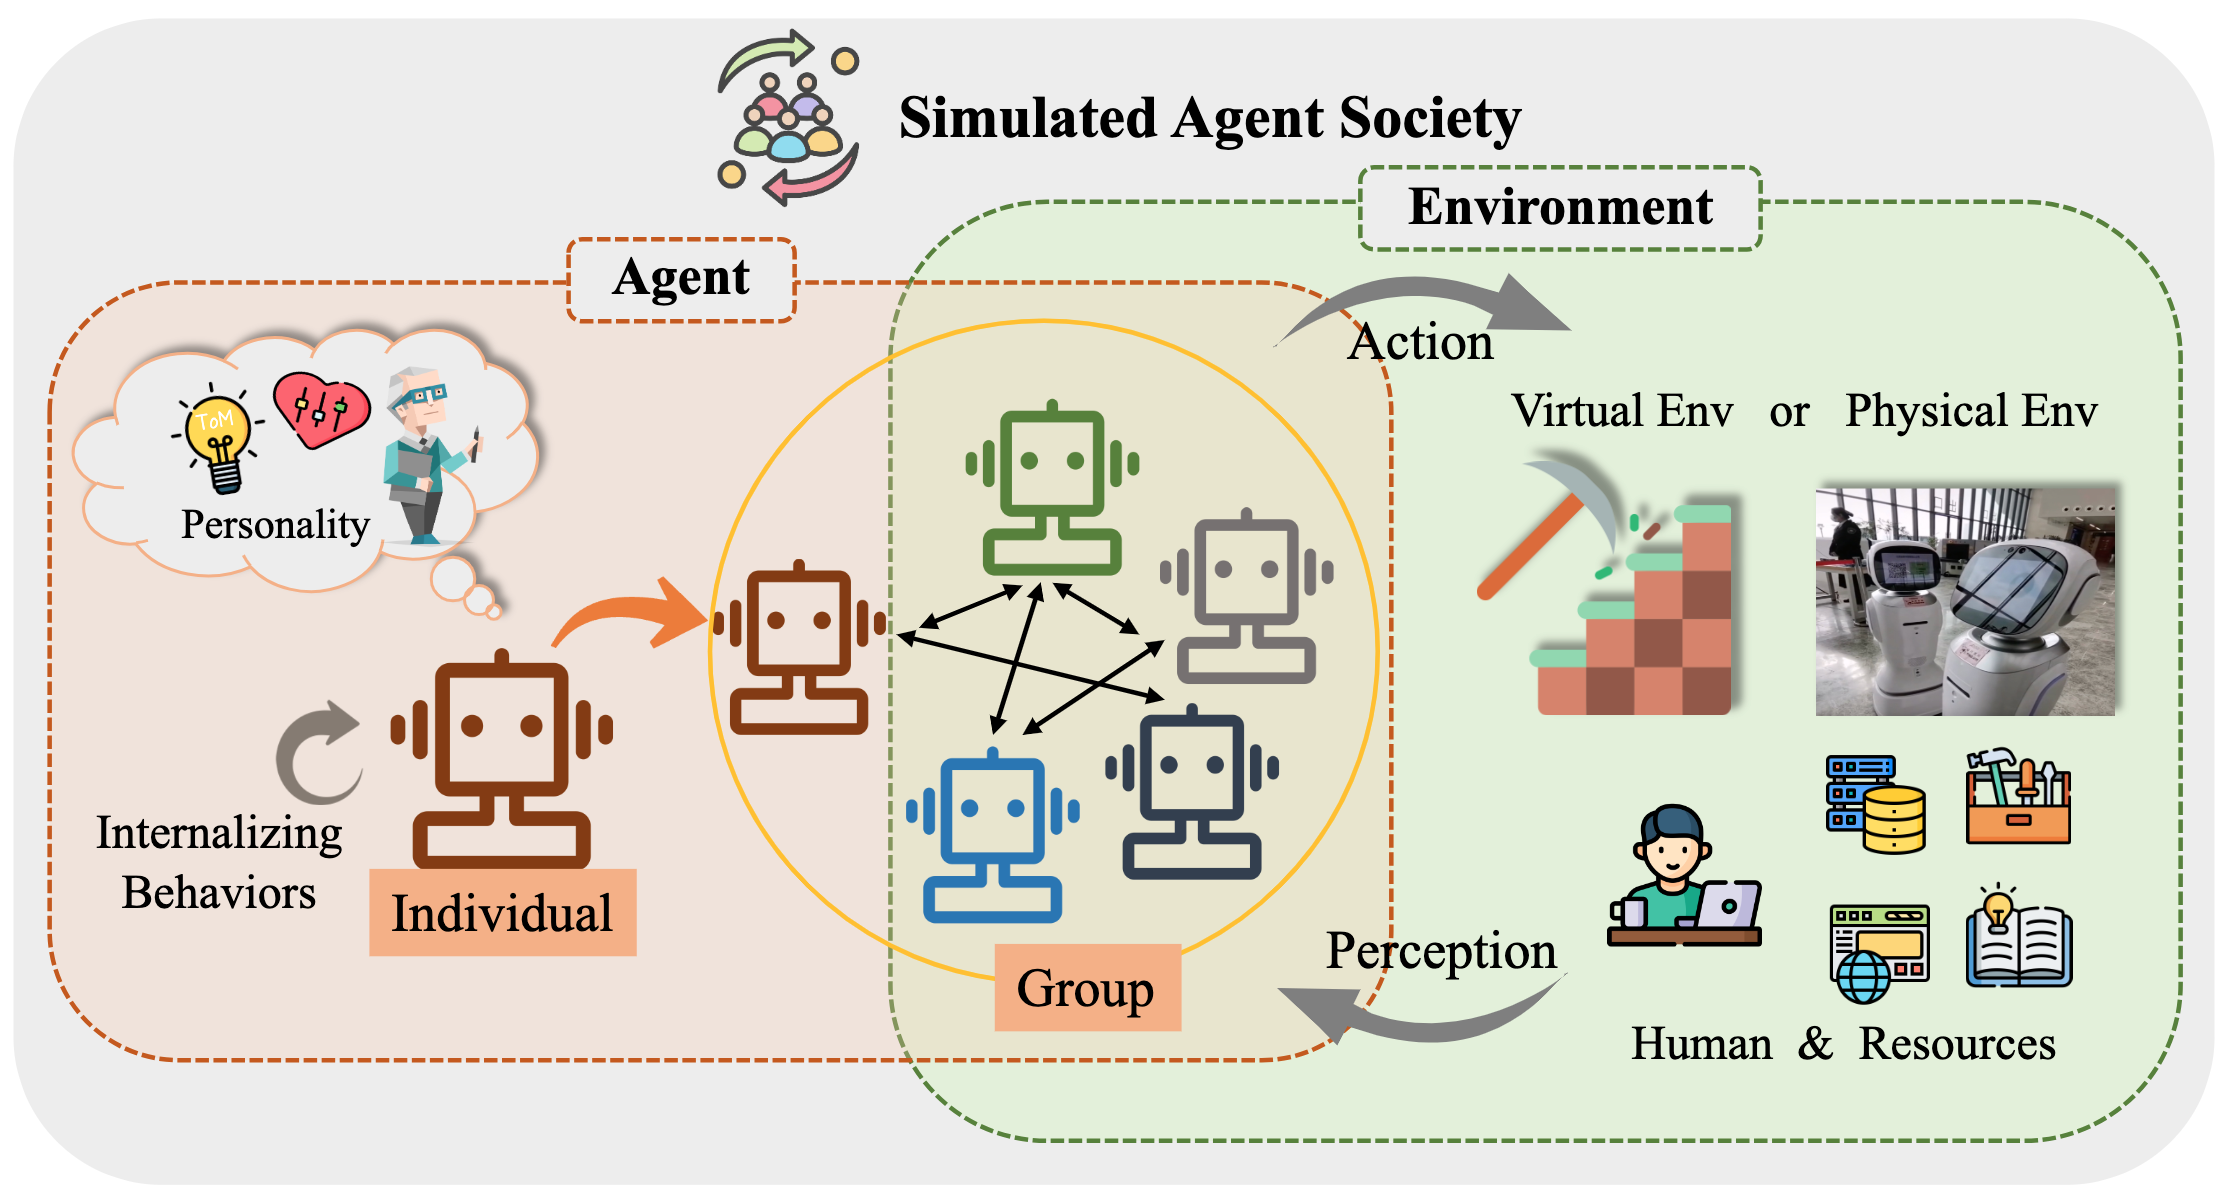
\includegraphics[width=0.8\textwidth]{image/figure12.jpg}
    \caption{Simulated Agent Society\cite{xi_rise_2023}}
  \label{fig:agent_society}
\end{figure}
Humans have long been pursuing Artificial Intelligence (AI) that equals or exceeds the human level, and AI agents are considered a promising vehicle for this pursuit. 
AI agents are artificial entities that are capable of perceiving their environment, making decisions, and taking actions. 
Due to the versatility and extraordinary capabilities demonstrated by Large Language Models (LLMs), they are seen as a potential spark for Artificial General Intelligence (AGI) and hold promise for building general-purpose AI agents\cite{xi_rise_2023}. 
Many research efforts have utilized LLMs as a basis for building AI agents and have made significant progress in simulating human behavior.
\begin{figure}
    \centering
    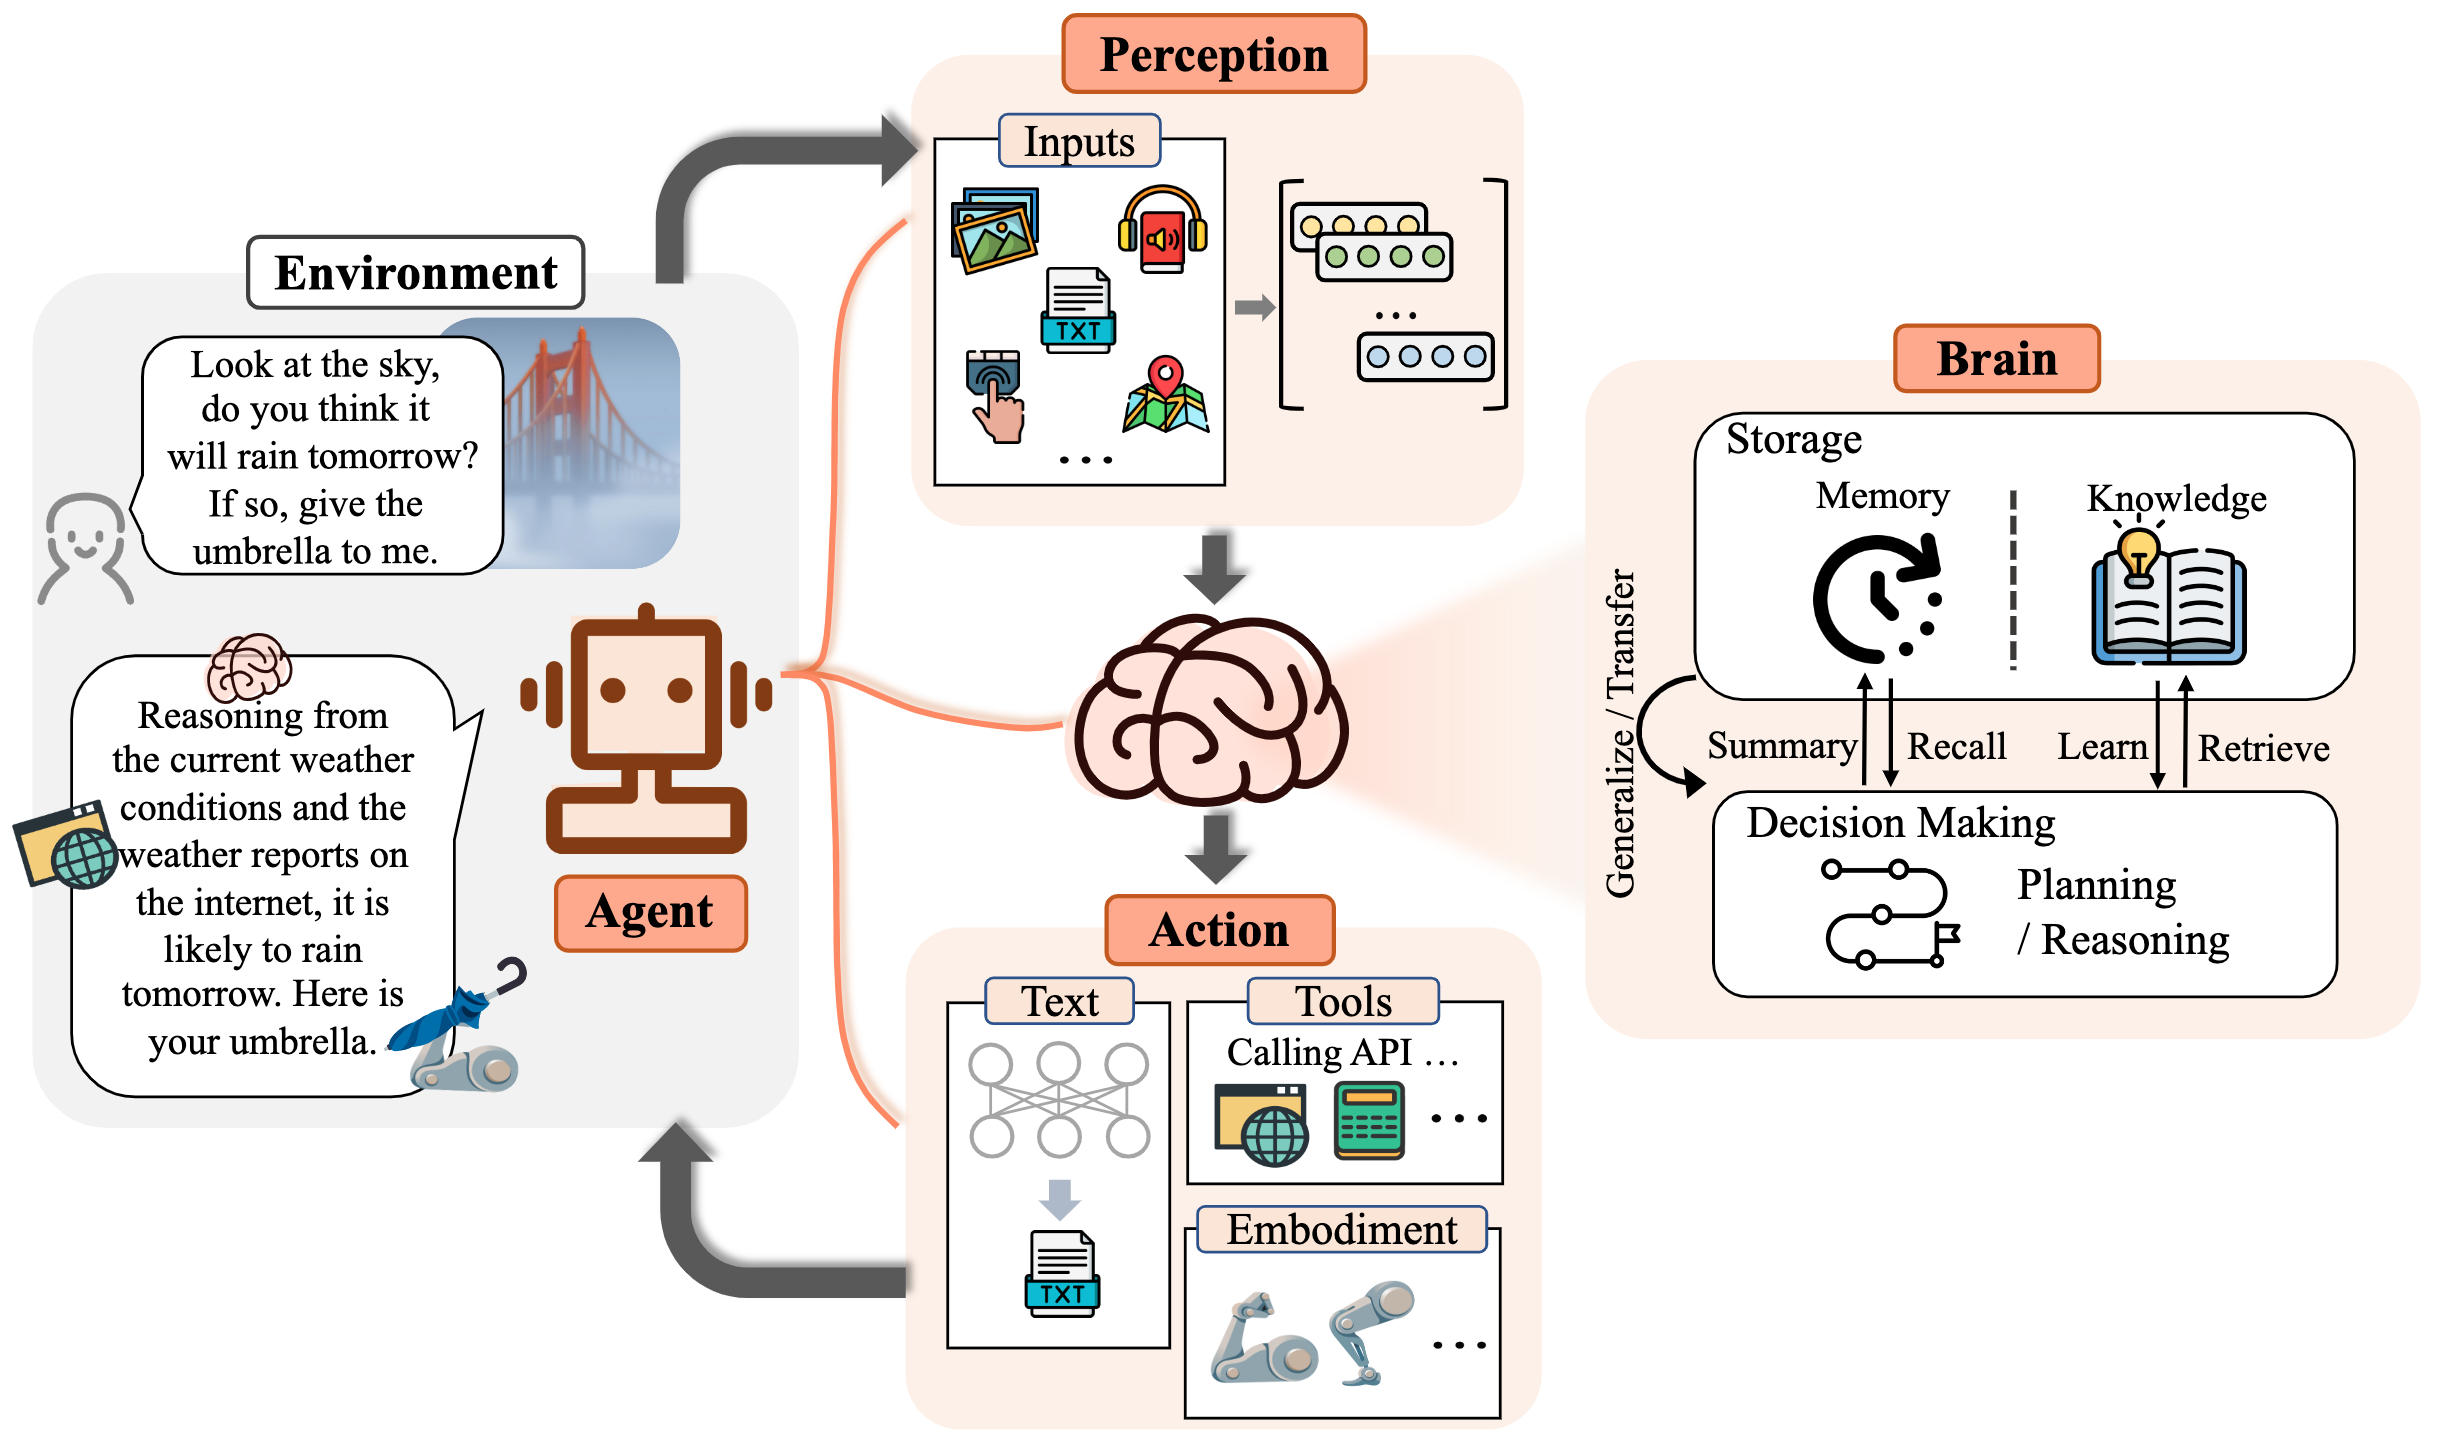
\includegraphics[width=0.8\textwidth]{image/figure2.jpg}
    \caption{Conceptual framework of LLM-based agent Conceptual framework of LLM-based agent with three components: brain, perception, and action. Serving as the controller, the brain module undertakes basic tasks like memorizing, thinking, and decision-making. The perception module perceives and processes multimodal information from the external environment, and the action module carries out the execution using tools and influences the surroundings.\cite{xi_rise_2023}}
  \label{fig:agent_conceptual_framework}
\end{figure}
Specifically, researchers employ LLMs as the primary component of brain or controller of these agents and expand their perceptual and action space through strategies such as multimodal perception and tool utilization\cite{yao2022react}.
These LLM-based agents can have certain reasoning and planning capabilities through techniques such as Chain of Thoughts (CoT) and problem decomposition, and can also learn and execute from feedback New actions are used to gain the ability to interact with the environment, and research has shown that allowing multiple agents to coexist may lead to the emergence of social phenomena\cite{park2023generative}.
Wang et al.\cite{wang_unleashing_2023} propose Solo Performance Prompting (SPP), which transforms a single LLM into a cognitive synergist by engaging in multi-turn self-collaboration with multiple personas.
Some research focuses on combining multiple agents through natural language and coding to try to solve practical problems\cite{chen_agentverse_2023, wu_autogen_2023}.
Chen et al.\cite{chen_gamegpt_2023} allow gpt to play different roles in the actual game production and development process, using different domain knowledge to take on corresponding responsibilities and jointly develop games.

\textbf{Problem Definition}\quad
My project focuses on developing a multi-agent artificial intelligence system for narrative gaming that not only simulates human behavior but is also designed for interactive storytelling. 
These specific research questions also came to light after the above-mentioned literature review.

\begin{itemize}
    \item [1)] 
    \textbf{How do artificial intelligence agents dynamically and autonomously perceive multimodal information within a virtual game space?} 
    This issue delves into the cognitive aspects of artificial intelligence agents, exploring the ways in which they process, interpret, and respond to different types of sensory information in their environment. The challenge is to create an agent that can effectively recognize and understand the various inputs in the game's virtual environment (such as visual cues, auditory signals, and textual data) and organize these inputs in a structured and rational manner.
    \item [2)]
    \textbf{How can artificial intelligence agents effectively use the information they sense to make dynamic decisions and plan tasks in virtual narrative game environments?} 
    This question explores the cognitive capabilities of artificial intelligence agents, focusing on their ability to translate collected sensory data into actionable strategies. The challenge here is to develop an agent that can not only understand the context of the game and evaluate the situation, but also predict potential outcomes and execute informed decisions that are consistent with the overall goals of the game. 
    This requires the creation of complex decision-making and planning algorithms that adapt to the dynamic nature of the game environment.
    \item [3)]
    \textbf{How to design and implement various forms of interaction between artificial intelligence agents and users in narrative metaverse games?} 
    This issue delves into the interactive aspects of artificial intelligence agents, focusing on how they engage users in meaningful and immersive ways. The challenge is to create an agent that understands user input, responds appropriately, and adjusts its behavior based on user actions while enhancing the narrative of the game.
\end{itemize}

\subsubsection{Objective and Scope of the Project}
The main goal of this project is to design and develop a multi-ai agent system for narrative games that is capable of simulating human behavior, interacting effectively with users, and contributing to immersive storytelling experiences. 
The system aims to push the boundaries of existing gaming technologies by introducing AI agents capable of autonomously perceiving and interpreting multimodal stimuli in virtual environments, utilizing the perceived information for dynamic decision making and task planning, 
and interacting with users in a diverse manner in narrative metaverse games. 
The project is broad in scope but focused, covering aspects of AI, game design and interactive narrative. 
After referring to the /textbf{"SMART"} criteria, i.e. \textit{Specific, Measurable, Achievable, Relevant} and \textit{Time-bound}, the Objective and Scope can be categorized as follows:

1. Develop an intelligent agent system that can perceive and interpret multimodal stimuli. 
This involves the construction of intricate perceptual algorithms capable of processing various information types within the virtual gaming landscape, 
methodically organizing and processing them. The AI agent should reliably detect environmental changes, identify crucial cues and external information, 
and react to this data in a manner aligning with the game's plot and objectives.

2. Construct an AI agent system that supports dynamic decision-making and task planning. 
The system devised should process perceived information to make decisions, steering the storyline dynamically based on these choices. 
This includes formulating sophisticated decision-making algorithms enabling them to comprehend the environment, assess different scenarios, anticipate potential results, and strategically plan tasks. 
The AI agent should demonstrate adaptability to the variable nature of the gaming environment and the player's actions.

3. Establish techniques for multiple intelligent agents to interact with users in narrative metaverse games. 
Artificial intelligent agents should be engineered to interface with the player in diverse ways that enrich the game's story and result in a captivating gaming experience. 
This necessitates the development of interactive algorithms capable of understanding user inputs, providing suitable responses, and modifying the agent's behavior based on user conduct.

\subsubsection{Research Method and Justification}
The rough components (preliminary idea) of the entire ai agent system for metaverse story-telling game are shown in the figure\ref{fig:system_mindimg}. 
It is not difficult to see that the left side is more focused on the information that the system should provide to the Large Language base model, including the external virtual environment、the character persona provided when perceiving and personalizing the character、 
the memory module that is defined in advance and dynamically generated and updated, and other game values serve the function. 
On the right side are the decision-making, planning and various interaction methods that we are eager to use the processing power of LLM to perform.
In traditional believable proxies of human behavior agent systems that do not include LLM, a similar perceive-plan-act cycles structure has been proven effective.
They maintained short-term and long-term memories, filled these memories with symbolic structures, and operated in perceive-plan-act cycles, dynamically perceiving the environment and matching it with one of the manually crafted action procedures\cite{umarov2012believable}. Agents created using cognitive architectures aimed to be generalizable to most, if not all, open world contexts and exhibited robust behavior for their time.
The parts highlighted in yellow in the picture are the scope of my research, and the following introduction to the research methods will also focus on these parts.

\begin{figure}
    \centering
    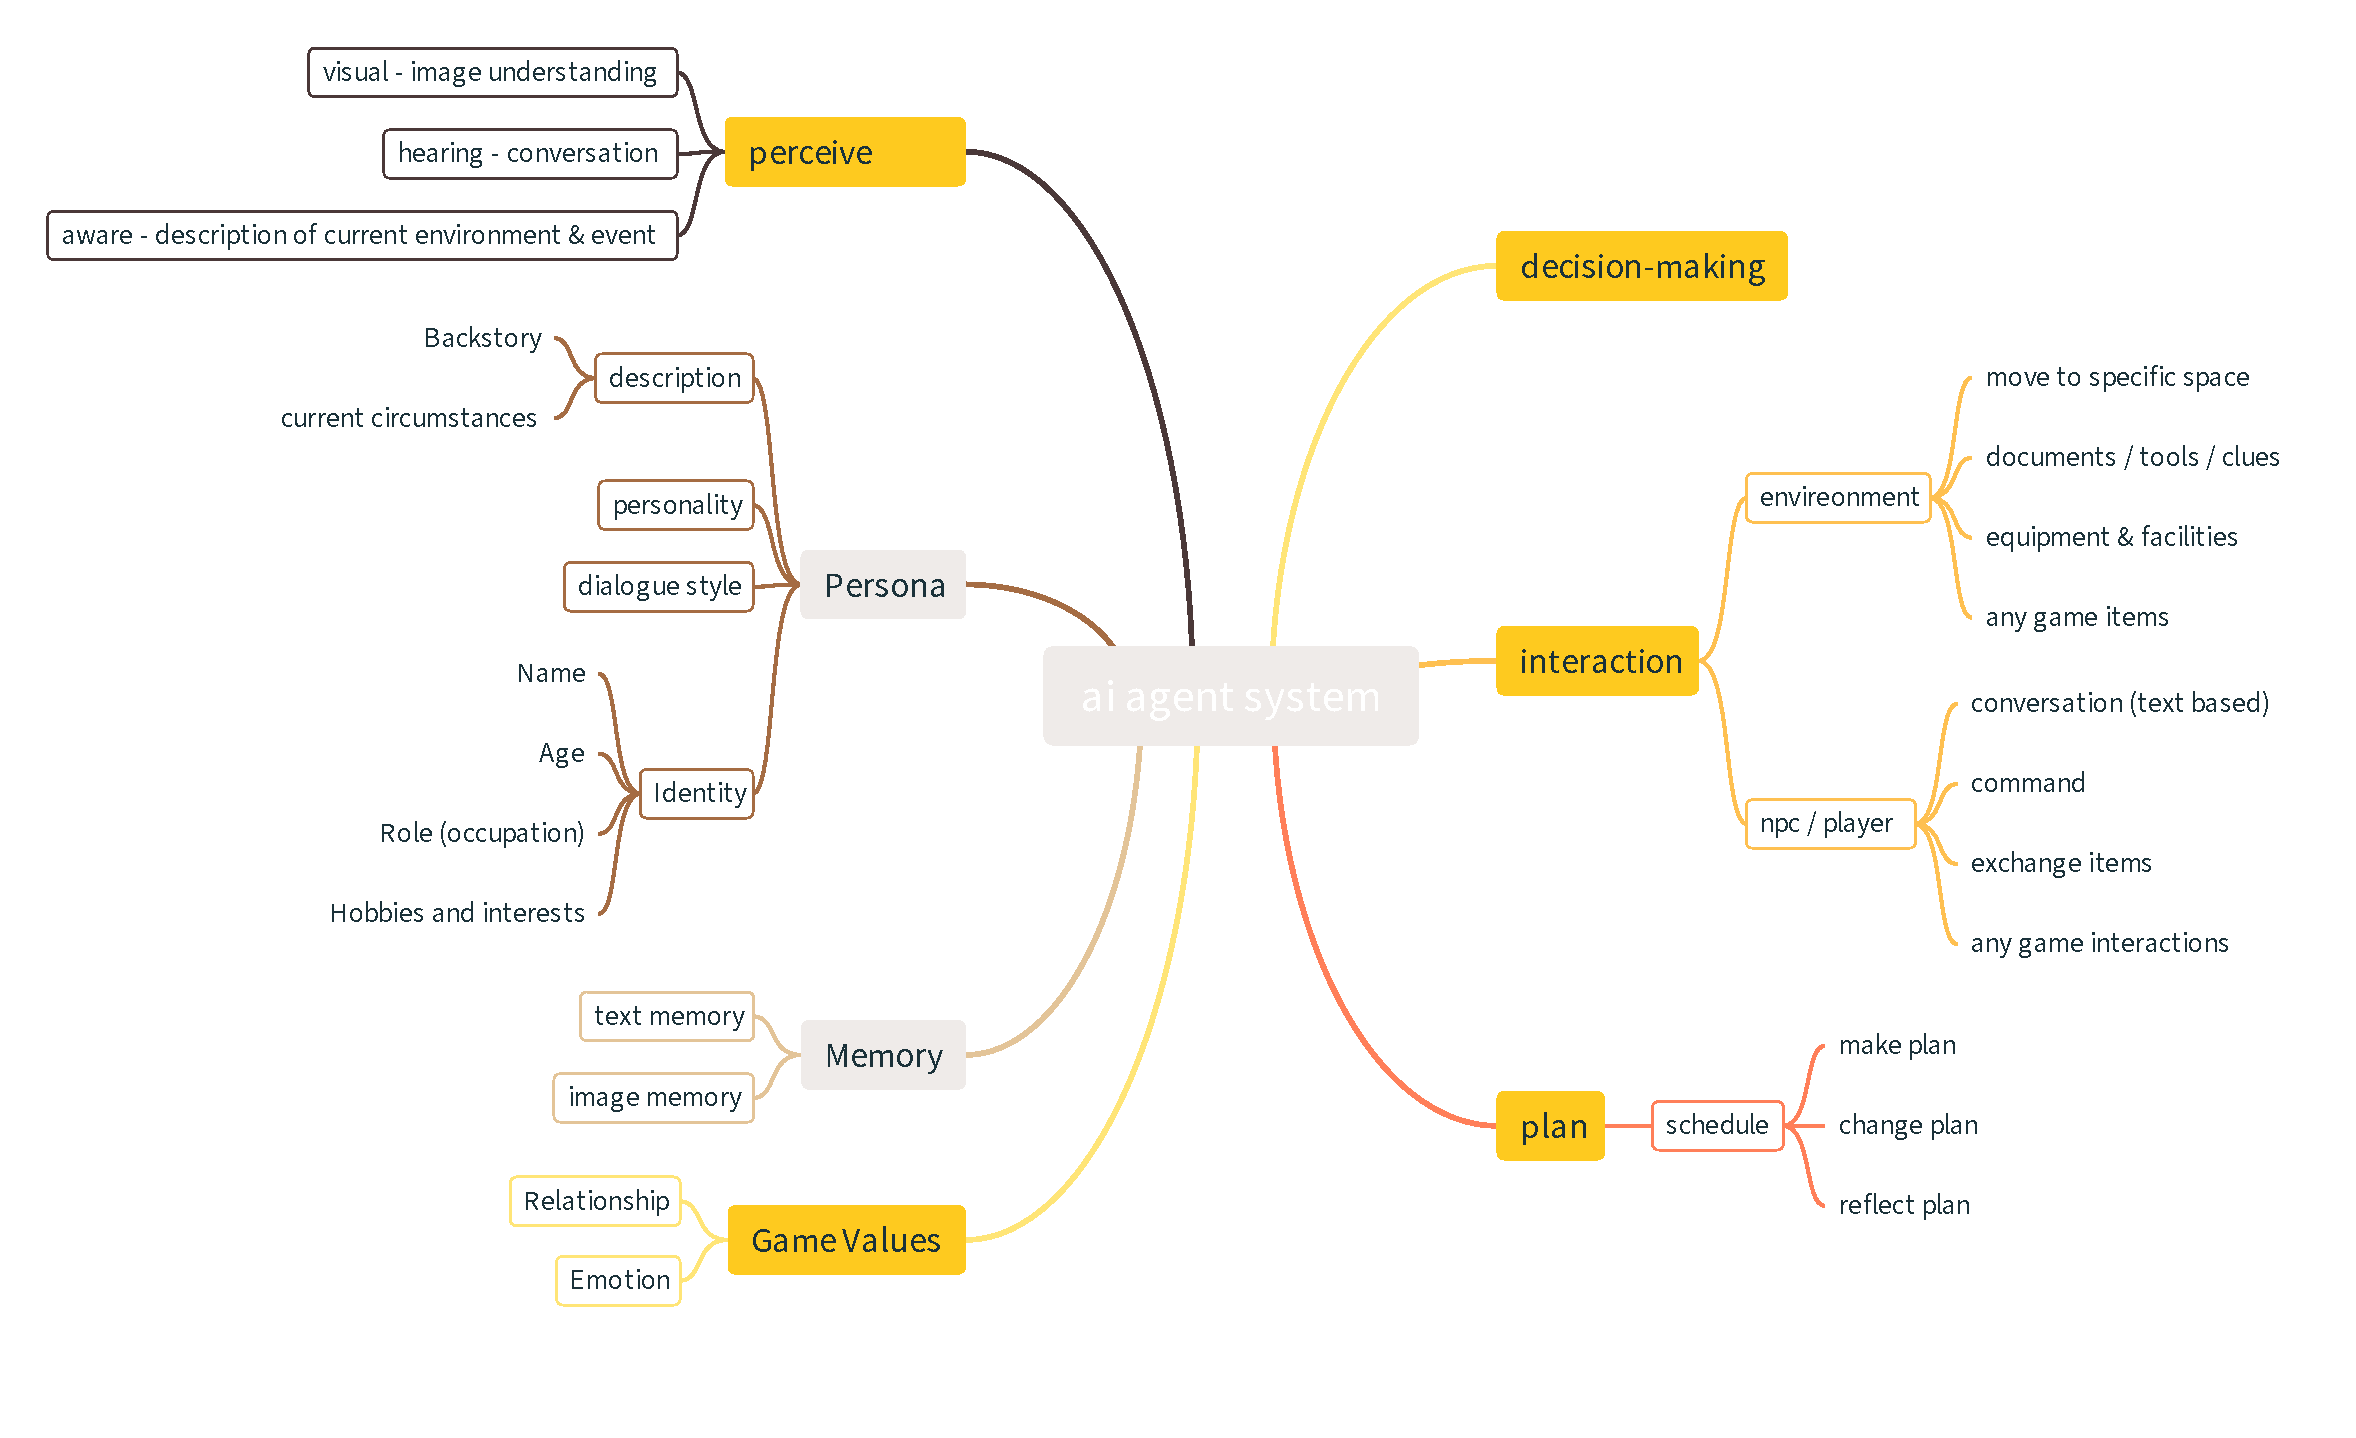
\includegraphics[width=0.8\textwidth]{image/system_mindimg.pdf}
    \caption{Ai Agent System Framework}
  \label{fig:system_mindimg}
\end{figure}

\textbf{Perceive}\quad
Both humans and animals rely on sense organs such as eyes and ears to gather information from their surroundings. 
These sensory inputs are converted into neural signals and sent to the brain for processing, allowing us to perceive and interact with the world. 
Likewise, it is crucial for LLM-based AI agent systems to receive information from various sources and ways. 
This expanded perceptual space can help agents better understand their environment, make informed decisions, and perform well on a wider range of tasks\cite{xi_rise_2023}. 
The Agent passes this information to the Brain module for processing through the perception module.
In the perception function module I designed, the main source of information is the NPC's natural perception of the internal environment of the game, that is, the description, numerical values and other information of the NPC's surrounding environment and events can be obtained directly from the game system. 
The visual information part will be handled by Guo, but how to obtain the image in the game system and where to input the extracted image information for processing are all issues that need to be designed and solved. 
This information will help the agent better perceive the external environment and is the cornerstone of dynamic decision-making and interaction.

\textbf{Game Values - Relationship}\quad
Interpersonal relationships should affect the decision-making or interaction style of a human behavioral agent. It is not only related to the identity and mentality changes in the narrative process, 
but also should have an impact on conversation style and decision-making, which will greatly promote the immersion of the user's experience.
Our Muiti-AI agent narrative system should be able to dynamically evaluate and change the relationship between users and agents based on the interactions and narrative interactions between them. 
In the context of this research project, Josselson's theory of relational development will be instrumental in shaping the AI's understanding and management of in-game relationships\cite{josselson1996space}. 
This theory, which identifies eight dimensions of interpersonal relationships as figure\ref{fig:relationship}, provides a comprehensive framework for simulating human-like interactions within the game.
\begin{figure}
    \centering
    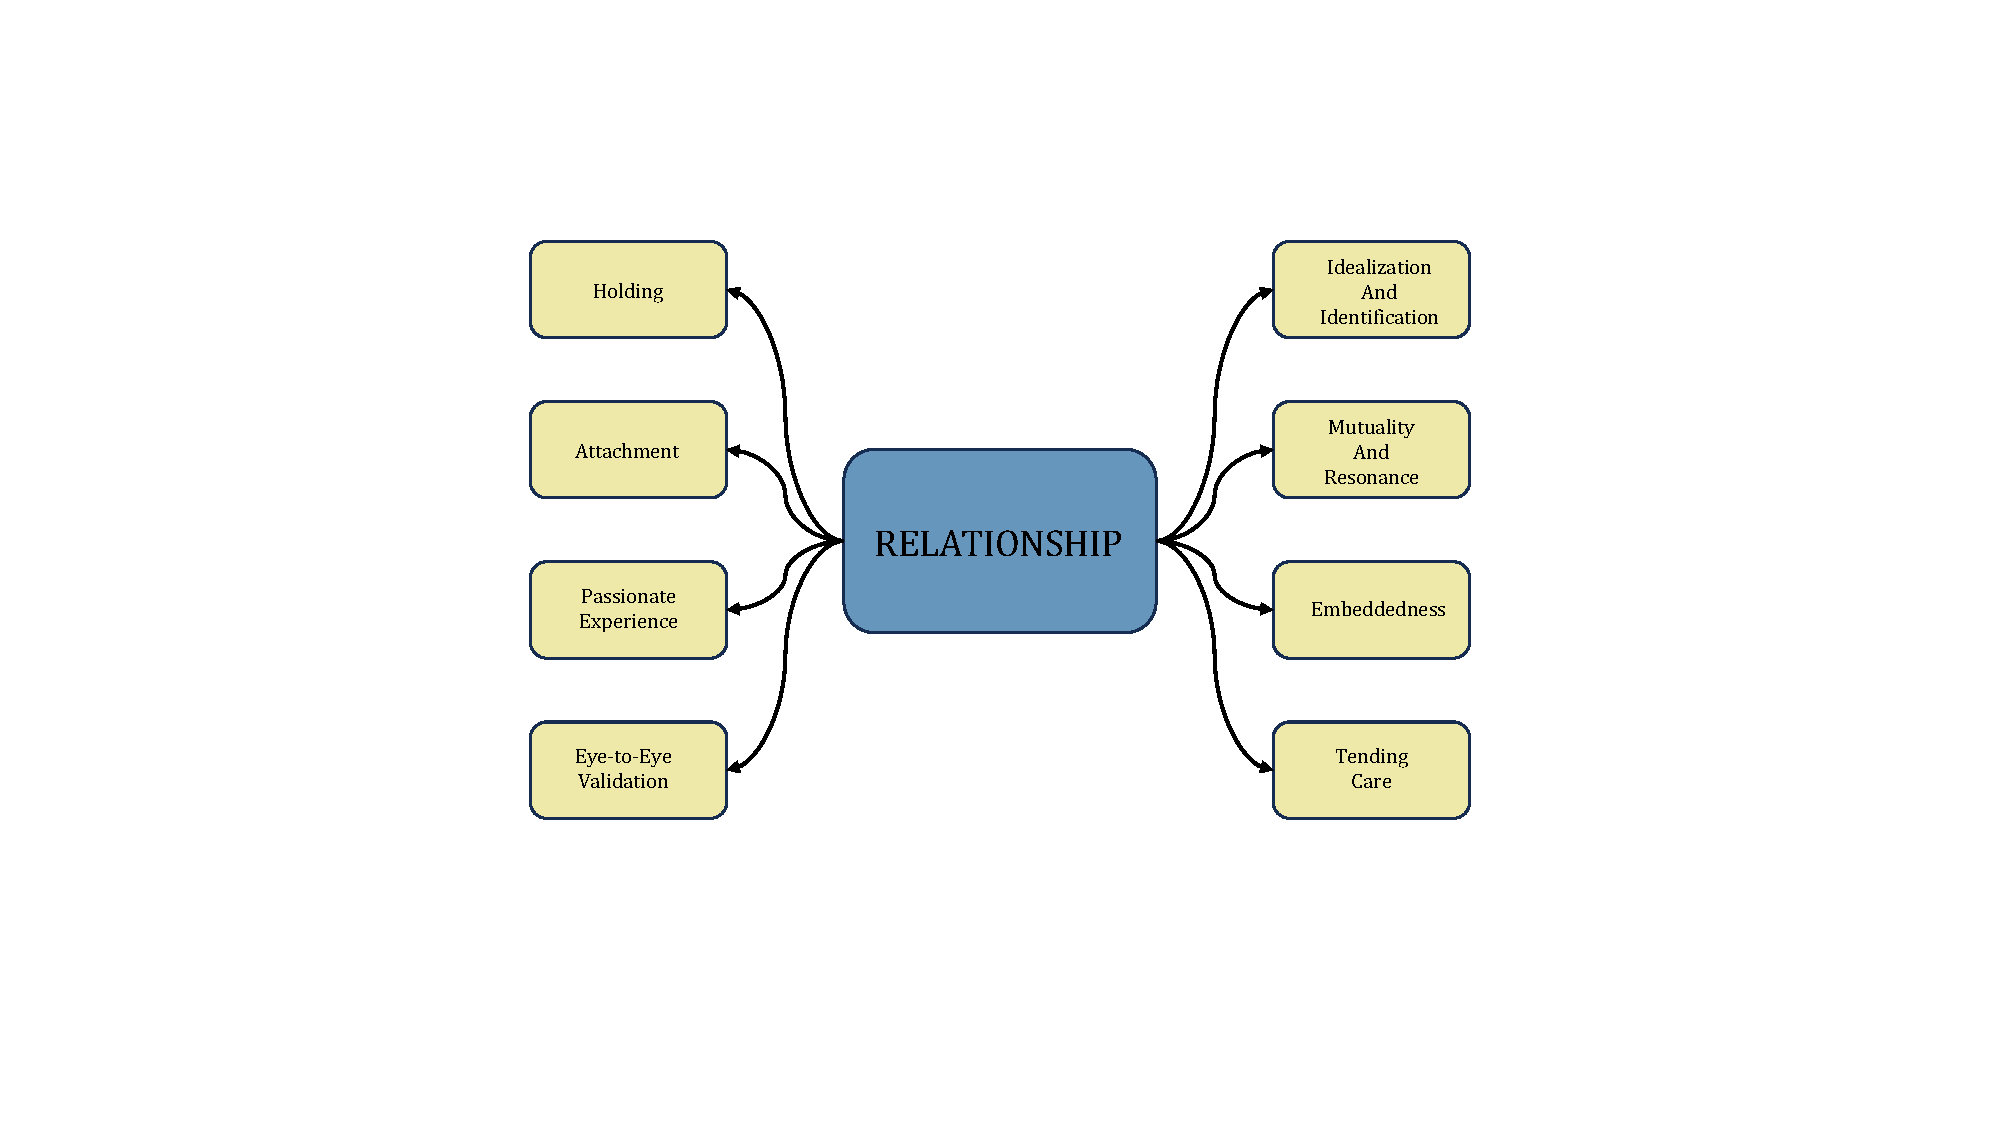
\includegraphics[width=0.8\textwidth]{image/relationship.pdf}
    \caption{eight dimensions of interpersonal relationships}
  \label{fig:relationship}
\end{figure}

\textbf{Game Values - Emotion}\quad
The Emotion component allows the AI agents to dynamicly understand, express, and respond to emotional interactions within the game. 
This component is grounded in psychological theories, particularly Plutchik's wheel of emotions as figure\ref{fig:emotions}, which identifies eight primary emotions: \textit{joy, trust, fear, surprise, sadness, disgust, anger}, and \textit{anticipation}\cite{plutchik1980general}. 
In the context of this research project, AI agents will be programmed to recognize and respond to these emotions within the game environment. 
This involves two key processes: perception and expression. AI agent might have the ability empowered by LLMs to change emotion when facing a character's dialogue or an event. 
Furthermore, the AI agent will be programmed to understand the context and cause of the emotion, which can be influenced by various factors such as the character's relationships, current events in the game, or the character's personal history. 
Expression, on the other hand, involves the AI's ability to portray emotions through the game characters. 
This is achieved by generating appropriate responses that align with the perceived emotion. 
For example, if an AI agent perceives that a character is experiencing fear, the agent might generate a response that involves the character seeking safety or expressing discomfort. 
By incorporating Plutchik's wheel of emotions, the AI agent system will be able to simulate a wide range of emotional experiences, adding depth and realism to the game narrative. 
This approach also enables the AI agents to understand the emotional dynamics within the game, which is crucial for making strategic decisions and fostering meaningful interactions. 
Moreover, the ability to understand and express emotions can significantly enhance the player's gaming experience. 
It allows for a more immersive and emotionally engaging narrative, where characters respond to events and each other in a human-like manner. 
\begin{figure}
    \centering
    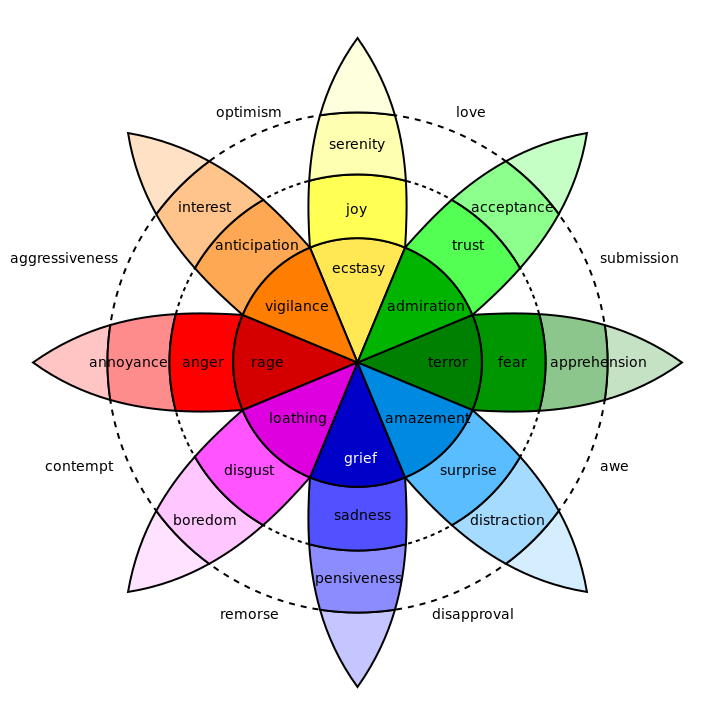
\includegraphics[width=0.8\textwidth]{image/Plutchik-wheel.png}
    \caption{Plutchik's wheel of emotions}
  \label{fig:emotions}
\end{figure}

\textbf{Decision-making \& Plan}\quad
The decision-making and planning components of an AI agent system are critical for the AI agent to be able to make decisions and plan tasks based on the information from the game system. 
As shown in the figure\ref{fig:decision-making}, the AI agent first collects and organizes information from the game environment, including the background, memory, personality, relationships, and emotions of the game characters. 
This information is crucial to understanding the current situation and making corresponding decisions. 
Based on the collected information, the artificial intelligence agent makes decision-making choices and outputs a corresponding text of personalized expression. 
This expression can reflect the impact of the various influencing factors mentioned above on the decision-making and is presented to the user and system in a specific interactive manner which are an important part of the entire dynamic interactive narrative that reflects user customization and enhances immersion. 
After confirming the selection, the AI agent performs the selected behavior. This may involve interacting with other characters, manipulating objects in the game world, or moving to different locations. 
Finally, the AI agent evaluates the consequences of its actions. This involves evaluating whether the action succeeds in achieving the goal and considering the impact of the action on the game world and character state. 
Based on this assessment, the AI agent may adjust its strategy and plan future actions. 
By integrating these steps into an artificial intelligence system, the project aims to enable artificial intelligence agents to autonomously navigate the game world, make decisions, and interact with other characters in meaningful ways. 
This approach enhances the authenticity and complexity of the game's narrative, providing players with a more engaging and immersive gaming experience.
\begin{figure}
    \centering
    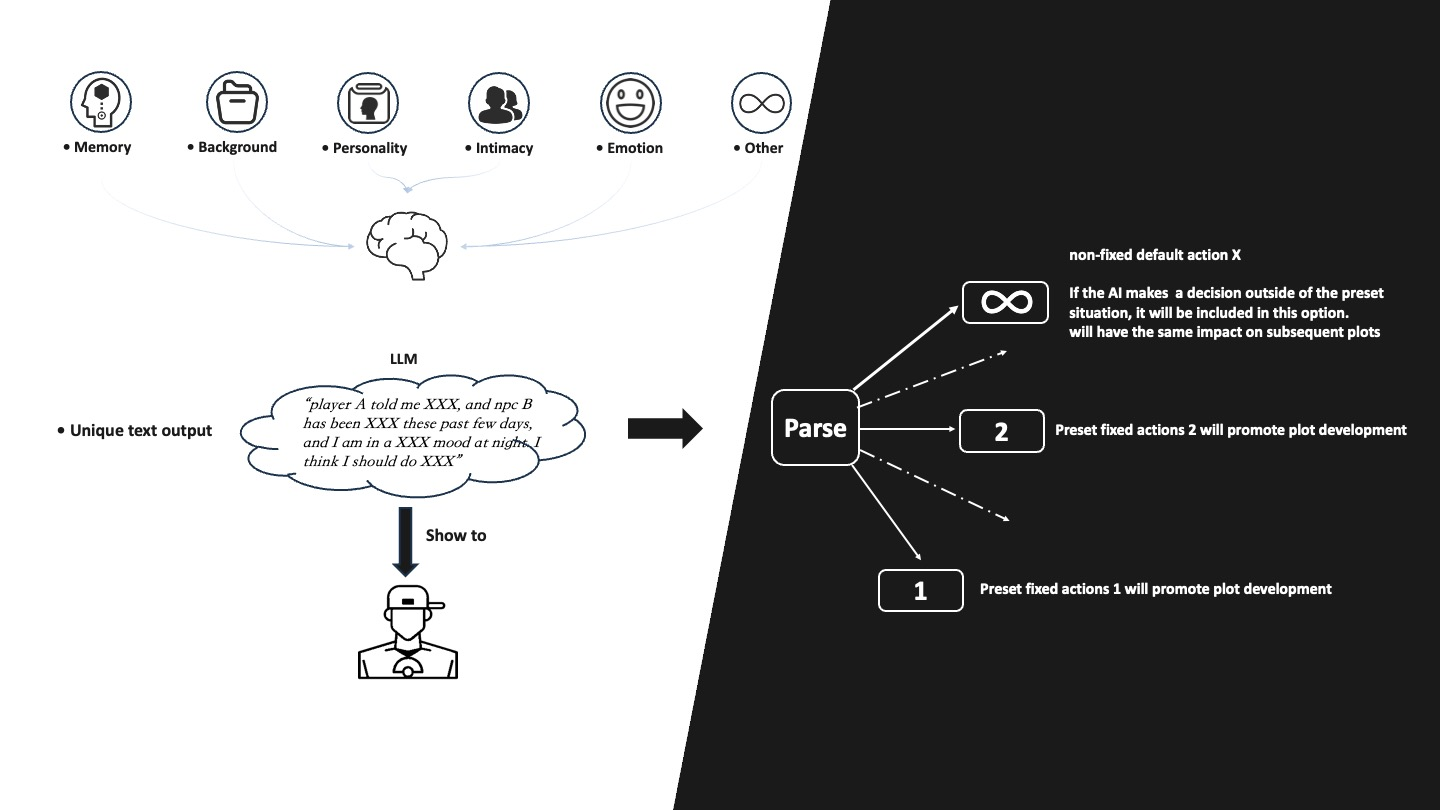
\includegraphics[width=0.8\textwidth]{image/decision-making.jpg}
    \caption{Decision-making Pipeline}
  \label{fig:decision-making}
\end{figure}

\textbf{Interaction}\quad
The interactive component of an AI agent system is critical to the overall gaming experience because it facilitates meaningful interactions between the AI agent and the game environment, 
as well as between the AI agent and other characters (whether other AI agents or human players). 
This process can be divided into two main parts: environment interaction and character interaction. 
Environment interaction: This involves the ability of an AI agent to effectively navigate and interact with a virtual space. 
This includes 1. AI agents should be able to move autonomously in the game world, traverse complex terrain and avoid obstacles. 
2. Object interaction: AI agents should be able to interact with various objects in the game world. 
This may involve picking up items, using tools, or examining clues. AI should understand the purpose and potential use of each object and use this knowledge to make strategic decisions. 
3. Facility interaction: In addition to objects, AI agents should also be able to interact with various facilities in the environment. 
These interactions can significantly impact the game's narrative and character progression. 
Character Interaction: This involves the ability of the AI agent to interact with other characters in the game. 
This includes: 1. Text-based dialogue: AI agents should be able to have meaningful conversations with other characters. 
This requires a sophisticated natural language processing system capable of understanding and generating text-based conversations. 
AI should be able to interpret the content, tone and emotion of a conversation and respond in a way that fits the character's personality and goals. 
2. Giving and receiving orders: AI agents may need to give or follow orders, especially in games involving team-based tasks or hierarchical relationships. 
This requires AI to understand the context of the command and perform the appropriate action. 
3. Exchange items or information clues: AI agents should be able to exchange items with other characters. This may involve giving or receiving items, or negotiating a deal. 
AI should understand the value and potential use of each project and use this knowledge to make strategic decisions.


\subsubsection{Execution Plan}

\textbf{Literature Review}\quad
This initial stage involves a thorough review of current research in areas related to AI in gaming, perception, decision-making, and narrative metaverse games. The aim is to understand the state-of-the-art techniques and methodologies, identify gaps in existing knowledge, and determine how this project can contribute to the field. The review should be systematic, including academic papers, technical reports, and other relevant publications.

\textbf{Framework Design}\quad
Based on the insights gained from the literature review, a detailed framework for the AI agent system should be designed. It involves outlining the system's architecture, defining the core components, and establishing the interfaces between these components. Each component's role and functions should be clearly defined, and the data flow between them should be mapped out.

\textbf{Game Environment \& Functional Module Development:}\quad
This stage involves two parallel processes: creating the game environment and developing the functional modules of the AI agent system. 
The game environment should be designed to provide a diverse set of stimuli and interaction possibilities for the AI. It should be rich in features, with varying landscapes, objects, and characters, to fully test the AI's capabilities. 
The development of the AI's functional modules should be done in a prioritized manner. 
The basic interaction and perception functions should be developed first. 
These modules will allow the AI to perceive its environment and interact with it. 
Once these are in place, the decision-making and planning modules can be developed. 
These modules will enable the AI to make strategic decisions and plan tasks based on its perceptions. 
Additional functionalities can be added in sequence, depending on the requirements of the game environment.

\textbf{System Integration}\quad
After the basic functional modules are developed, they should be integrated into a cohesive system. 
This involves ensuring that the modules work together effectively, with data flowing seamlessly from perception to decision-making to interaction. 
Any inconsistencies or errors in data flow should be rectified at this stage.

\textbf{Testing and Evaluation}\quad
Unit Testing: Each functional module should be tested individually to ensure it performs its specific tasks correctly. This can involve feeding the module a set of inputs and verifying that it produces the expected outputs. 
System Testing: Once all modules are integrated, the entire system should be tested. This involves running the AI in the game environment and observing its behavior to ensure it perceives, decides, and interacts as expected. 
Performance Testing: The AI should be tested under different conditions to assess its performance. This can involve changing the game environment, altering the AI's goals, or introducing unexpected events. 
Usability Testing: This involves testing the AI from a player's perspective. This can involve observing how players interact with the AI, gathering their feedback, and making necessary adjustments to improve the gameplay experience.

\textbf{Iterative Improvement}\quad
Iterative refinement and improvement of the AI agent system based on the results of testing and evaluation. 
This includes identifying weaknesses in the system, making necessary adjustments, and retesting the system. 
At the same time, if necessary, real user testing will be introduced to collect real user feedback data and information, and iterative products will be repeatedly updated based on user research, and technical details and design structures will be continuously improved. 
The goal is to continuously enhance the capabilities of the AI agent system and the overall gaming experience.

\textbf{Documentation \& Publication}\quad
Finally, research results should be carefully documented and published. This includes detailing the design and development process, outlining test and evaluation results, and discussing the potential implications and future directions of the research. 
Research results should be disseminated in relevant academic journals, conferences and other appropriate platforms.


\subsubsection{Intended Outcomes}

\textbf{Outcome 1: Creation of an AI Agent System Capable of Multimodal Perception Interaction and Dynamic Decision-Making}\quad
This outcome involves the development of a sophisticated AI agent with the ability to perceive and interpret multimodal stimuli within a virtual game environment. 
The AI agent, equipped with advanced algorithms, will be able to process visual, auditory, and other forms of sensory input. 
The agent will be designed to understand the essence of the environment, including the attributes of different objects, the spatial relationships between them, and the dynamics of their interactions. 
Beyond perception, the AI agent will be able to make strategic decisions based on its understanding and dynamically plan tasks to interact with the environment. 
The agent's decision-making process will be designed to emulate human-like cognition, considering multiple factors, evaluating potential outcomes, and making decisions in a dynamic, evolving game environment.
This AI agent system forms the core of the group project's objective - creating an AI-driven storytelling game in the Metaverse. The agent's ability to perceive the game environment and make strategic decisions will drive the game's narrative and provide a dynamic and engaging player experience. 
The individual project will determine the depth and richness of the game's narrative and the level of interaction possible for the players.

\textbf{Outcome 2: Integration of AI Agents into the Narrative Game Experience}\quad
Integrating the AI agent into a narrative game experience is not merely a technical integration, but also one that requires careful narrative design. The AI agent will not be a mere tool or mechanism in the game, but a character that contributes to the story. 
The agent could take on various roles within the narrative, and the AI's actions, decisions, and interactions will influence the course of the story, creating a unique narrative experience for each player. 
The AI will also be designed to adapt to the players' actions and decisions, providing a truly interactive storytelling experience.
The integration of the AI agent into the narrative game experience is a crucial aspect of the group project. It brings together the AI technology and the narrative design to create a unique game experience in the Metaverse. 
It showcases the project's innovative approach to game design, where the story is not fixed but evolves dynamically based on the AI's decisions and the player's interactions.

\textbf{Outcome 3: Advancement in AI-driven Storytelling in the Metaverse}\quad
This outcome represents a significant advancement in the field of AI-driven storytelling in the Metaverse. 
The project will demonstrate how AI technology can be used to drive narrative in a virtual game environment, providing a dynamic, interactive, and immersive storytelling experience. 
It will explore new possibilities for game design, where the narrative is not fixed but evolves based on the AI's decisions and the player's interactions. 
This could pave the way for more innovative uses of AI in gaming and broader applications in the Metaverse.
This advancement is the ultimate goal of the group project. By demonstrating the potential of AI-driven storytelling in the Metaverse, 
the project contributes to the broader field of AI in gaming, pushing the boundaries of what is possible in narrative game design. 
It represents a significant step forward in creating more interactive and immersive experiences in the Metaverse, opening up new possibilities for future game development.

%  -----  2.3
\subsection{Project Milestones}
Table the group project and the individual project milestones. 
Illustrate the relation and alignment of milestones of the individual project and those of the group project.

\begin{table}
    \renewcommand{\arraystretch}{3}
    \begin{center}
  \def~{\hphantom{0}}
    \begin{tabular}{lccc}
        \hline
        \textbf{Time}  & \textbf{Group-milestones} & \textbf{Individual-milestones}\\[3pt]
        \hline
         31/05/2024   & \makecell[c]{Development and initial testing of \\individual functional modules} & \makecell[c]{Preliminary development \\and testing of basic game environment \\and basic perceptual interaction functions}\\
         30/09/2024   & \makecell[c]{First generation prototype \\integration of basic functional modules} & \makecell[c]{Integration of basic game environment \\and basic perceptual interaction functions}\\
         31/03/2025   & \makecell[c]{Second Generation Prototype \\Optimized Integration and Narrative Development} & \makecell[c]{Development and integration of decision-making \\and planning functions}\\
         31/08/2025   & \makecell[c]{Third Generation Prototype \\Further Development, User Testing, and Iterative Optimization} & \makecell[c]{Testing, Evaluation \\and Iterative Improvement}\\
         \hline
    \end{tabular}
    \caption{Group and Individual Project Milestones}
    \label{tab:milestones2}
    \end{center}
\end{table}

\begin{itemize}
    \item [1)] 
    \textbf{May 31, 2024 - Preliminary development and testing of basic game environment and basic perceptual interaction functions:} 
    Group milestone focus on the development and initial testing of the various functional modules that make up the AI-driven narrative game. 
    Personal projects are consistent with this stage and focus on the development and testing of basic game environments and basic perceptual interaction functions. 
    This ensures that individual work on perception and interaction modules is synchronized with team efforts to build the underlying capabilities of the AI agent.
    \item [2)]
    \textbf{September 30, 2024 - Integration of basic game environment and basic perceptual interaction functions:} 
    Group milestone focus on integrating the basic functional modules developed by each member into the first generation prototype. 
    This includes combining the capabilities of AI agent systems with narrative structures to create interactive experiences. 
    Individual project milestone complement this by combining the developed base game environment with perceptual interaction features. 
    This ensures that individual work contributes directly to the prototype, enabling the AI agent to interact with users and the game environment in meaningful and easily demonstrable ways, while also integrating the milestones of other members.
    \item [3)]
    \textbf{March 31, 2025 - Development and integration of decision-making and planning functions:} 
    Group milestone aims to optimize the integration of functional modules and enhance the development of narrative. 
    The team worked to refine the prototype, resolve any issues with the first integration, and improve the interactive storytelling experience for players. 
    The focus of personal milestones at this stage is the development and integration of decision-making and planning functions to make up for the lack of decision-making and planning functions of the first-generation prototype. 
    This advancement of the personal project is critical to achieving more complete, complex, and responsive AI agents, while also helping to deliver richer narrative experiences that support the group’s narrative development goals.
    \item [4)]
    \textbf{August 31, 2025 - Testing, Evaluation and Iterative Improvement} 
    The final milestone for the group involves refining the game through user testing, gathering feedback and implementing iterative optimizations. 
    This stage is critical to ensuring the game resonates with users and provides an engaging experience. 
    In keeping with the team's goals, individual projects focus on testing, evaluating, and iteratively improving developed features. 
    This includes fine-tuning the decision-making and planning capabilities of the AI agent based on user feedback, ensuring that individual contributions improve the overall quality and appeal of the game.
\end{itemize}

%  -----  2.4
\subsection{Budget Plan}

\subsubsection{Estimated Budget}
The estimated budget for the project is about 35000RMB.

\subsubsection{Budget Breakdown}

\begin{itemize}
    \item \textbf{Equipment Expense:} 
    None.
    \item \textbf{Consumable Expense:} 
    There are some purchasing expenses in order to build a metaverse game system. One monitor costs about 1500RMB. 
    A GPU costs about 6000RMB, a CPU and mainboard costs about 3000RMB, and other related components 1500RMB. 
    \item \textbf{Testing and Processing Expense:} 
    The GPT-3.5/GPT-4 API service is used for early construction experiments and improvements which takes about 2000RMB.
    \item \textbf{Fuel and Power Expense:} 
    None.
    \item \textbf{Business Trip / Conference/ International Cooperation \& Exchange Expense} 
    16000 RMB.
    \item \textbf{Publishing/ Literature/ Information Dissemination/ Intellectual Property Expense} 
    5000 RMB.
    \item \textbf{Service Fee} 
    None.
    \item \textbf{Manpower Cost} 
    None.
    \item \textbf{Service Fee} 
    None.
    \item \textbf{Expert Consultant Expense} 
    None.
    \item \textbf{Other Expenses} 
    None.
    \item \textbf{Indirect Expense} 
    None.
\end{itemize}

\subsubsection{Cost-Effectiveness}
The budget breakdown reveals a thoughtful allocation of funds across various categories, taking into account the necessities for equipment, consumables, testing, processing, business trips, conferences, international cooperation, publishing, literature, information dissemination, and intellectual property expenses. 
The consumable expenses, primarily centered around the acquisition of components for building the metaverse game system, showcase a balance between quality and cost. 
Each component's cost has been carefully considered, with an eye towards obtaining the necessary hardware at an optimal price point. 
Testing and processing expenses are allocated for utilizing the GPT-3.5/GPT-4 API service, demonstrating a cost-effective strategy for early construction experiments and improvements. 
This API service provides a valuable resource for the project's development, offering a scalable and efficient solution. 
The budget also accounts for business trips, conferences, international cooperation, and exchange expenses, emphasizing the importance of collaboration and knowledge-sharing. 
Publishing, literature, information dissemination, and intellectual property expenses are allocated to ensure effective communication and protection of project outcomes. 
Overall, the budget demonstrates a judicious balance between essential expenses and the goal of maximizing the project's impact. 
By carefully allocating resources and prioritizing cost-effectiveness, the project aims to achieve its objectives in an efficient manner, ensuring that every allocated RMB contributes significantly to the advancement of the metaverse narrative game system.

%  -----  2.5
\subsection{Risk Analysis and Mitigation}

\subsubsection{Potential Risks or Challenges}
During the implementation of any project, it is crucial to identify potential risks or challenges and develop corresponding mitigation measures. 
Here are some potential risks we may encounter when developing an AI agent-driven narrative game in Metaverseon:

\begin{itemize}
    \item [1)] 
    \textbf{Technical Complexity and Integration Issues} 
    The integration of individual functional modules may be more complex than expected, causing delays and performance issues.
    \item [2)]
    \textbf{Software and Hardware Compatibility} 
    With the rapid development of technology, software and hardware compatibility issues may arise.
    \item [3)]
    \textbf{User Acceptance and Feedback} 
    Users may not accept new game mechanics or storytelling, which may affect the success of the game system.
    \item [4)]
    \textbf{AI agent’s perception and decision-making} 
    AI agents may not be able to accurately perceive the environment or make logical decisions, thereby degrading the gaming experience.
    \item [5)]
    \textbf{Project Management and Timeline Delays} 
    Projects may be delayed due to improper resource allocation, wrong priority setting, or unexpected challenges.
    \item [6)]
    \textbf{Data Privacy and Security} 
    Sensitive data may be involved in online games, and there is a risk of being hacked or data leaked.
    \item [7)]
    \textbf{Budget Overrun} 
    Project costs may exceed budget, especially if the development cycle is long and technology requirements are high.
\end{itemize}

\subsubsection{Impact of the Risks}

\begin{itemize}
    \item [1)] 
    \textbf{Technical Complexity and Integration Issues} 
    Impact Assessment: If functional module integration fails, it may cause project delays, increase costs, and reduce product quality. This could seriously impact a project's market launch time and competitiveness.
    Mitigation Strategy: Implement agile development methods and conduct regular small-scale incremental integrations so that issues can be discovered and resolved in a timely manner. Maintain strong communication between development teams and provide cross-module training to team members to enhance understanding and collaboration.
    \item [2)]
    \textbf{Software and Hardware Compatibility} 
    Impact Assessment: Compatibility issues may lead to inconsistent user experiences and limit game accessibility, thereby impacting user base and revenue.
    Mitigation Strategy: Develop cross-platform solutions and start testing on different devices and operating systems early in the development cycle. Also, set aside time and resources to resolve compatibility issues.
    \item [3)]
    \textbf{User Acceptance and Feedback} 
    Impact Assessment: Ignoring user feedback can result in a product that is inconsistent with market needs, reducing user satisfaction and engagement.
    Mitigation Strategy: Ensure user needs and expectations are understood through ongoing user engagement and testing cycles. Adjust game design based on feedback to ensure the game matches user expectations.
    \item [4)]
    \textbf{AI agent’s perception and decision-making} 
    Impact Assessment: If the perception and decision-making functions of the AI agent are inaccurate, it may destroy the user's immersion and gaming experience, thus affecting the appeal of the product.
    Mitigation Strategy: Use advanced AI technology and algorithms, conduct extensive training and testing to ensure the naturalness and adaptability of AI behavior. The AI system is regularly updated to adapt to new game content and user behavior.
    \item [5)]
    \textbf{Project Management and Timeline Delays} 
    Impact Assessment: Timeline delays may result in increased project costs, reduced return on investment, and possible loss of market opportunities.
    Mitigation Strategy: Develop a detailed project plan and timeline and track it using project management tools. Set up buffers for potential risks and develop contingency plans to deal with unforeseen events.
    \item [6)]
    \textbf{Data Privacy and Security} 
    Impact Assessment: A data breach or security incident can result in a loss of user trust, legal action, and long-term damage to a company's reputation.
    Mitigation Strategy: Implement a comprehensive security strategy including encryption, access control, and regular security audits. Provide user education that emphasizes the importance of security practices and data privacy.
    \item [7)]
    \textbf{Budget Overrun} 
    Impact Assessment: Going over budget can result in a shortage of funds, forcing the project to reduce scope, reduce quality, or cancel it entirely.
    Mitigation Strategy: Implement strict financial management and monitoring mechanisms. Conduct regular cost analysis and budget reviews and include risk reserves in project budgets.
\end{itemize}